%%%%%%%%%%%%%%%%%%%%%%%%%%%%%%%%%%%%%%%%%%%%%%%%%%%%%%%%%%%%%%%%%%%%%%%%%%%%%%%
\documentclass[hyperref={pdfpagelabels=false},compress,table]{beamer} % 在Mac下无法编译
% \documentclass[compress,table]{beamer} % 在Mac下使用
% package for font
\usepackage{fontspec}
\defaultfontfeatures{Mapping=tex-text}  %%如果没有它,会有一些 tex 特殊字符无法正常使用,比如连字符。
\usepackage{xunicode,xltxtra}
\usepackage[BoldFont,SlantFont,CJKnumber,CJKchecksingle]{xeCJK}  % \CJKnumber{12345}: 一万二千三百四十五
\usepackage{CJKfntef}  %%实现对汉字加点、下划线等。
\usepackage{pifont}  % \ding{}
% package for math
\usepackage{amsfonts}

% package for graphics
\usepackage[americaninductors,europeanresistors]{circuitikz}
\usepackage{tikz}
\usetikzlibrary{plotmarks}  % placements=positioning
\usepackage{graphicx}  % \includegraphics[]{}
\usepackage{subfigure}  %%图形或表格并排排列
% package for table
\usepackage{colortbl,dcolumn}  %% 彩色表格
\usepackage{multirow}
\usepackage{multicol}
\usepackage{booktabs}
% package for code
\usepackage{fancyvrb}
\usepackage{listings}

% \usepackage{animate}
% \usepackage{movie15}

%%%%%
% setting for beamer
\usetheme{default} % Madrid(常用), Copenhagen, AnnArbor, boxes(白色), Frankfurt,Berkeley
\useoutertheme[subsection=true]{miniframes} % 使用Berkeley时注释本行
\usecolortheme{sidebartab}
\usefonttheme{serif}  %%英文使用衬线字体
% \setbeamertemplate{background canvas}[vertical
% shading][bottom=white,top=structure.fg!7] %%背景色,上25%的蓝,过渡到下白。
\setbeamertemplate{theorems}[numbered]
\setbeamertemplate{navigation symbols}{}  %% 去掉页面下方默认的导航条
\setbeamercovered{transparent}  %设置 beamer 覆盖效果

% 设置标题title背景色
% \setbeamercolor{title}{fg=black, bg=lightgray!60!white}
\setbeamercolor{title}{fg=white, bg=black!70!white}

% 设置每页小LOGO
\pgfdeclareimage[width=1cm]{ouc}{figures/static/ouc.pdf}
\logo{\pgfuseimage{ouc}{\vspace{-20pt}}}

% setting for font
%%\setCJKmainfont{Adobe Kaiti Std}
\setCJKmainfont{SimSun} 
%% \setCJKmainfont{FangSong_GB2312} 
%% \setmainfont{Apple Garamond}  %%苹果字体没有SmallCaps
\setCJKmainfont{SimSun} 
%FUNNY%\setCJKmainfont{DFPShaoNvW5-GB}  %%华康少女文字W5(P)
%FUNNY%\setCJKmainfont{FZJingLeiS-R-GB}  %%方正静蕾体
%FUNNY%\setmainfont{Purisa}
%\setsansfont[Mapping=tex-text]{Adobe Song Std}
     %如果装了Adobe Acrobat,可在font.conf中配置Adobe字体的路径以使用其中文字体。
     %也可直接使用系统中的中文字体如SimSun、SimHei、微软雅黑等。
     %原来beamer用的字体是sans family;注意Mapping的大小写,不能写错。
     %设置字体时也可以直接用字体名,以下三种方式等同:
     %\setromanfont[BoldFont={黑体}]{宋体}
     %\setromanfont[BoldFont={SimHei}]{SimSun}
     %\setromanfont[BoldFont={"[simhei.ttf]"}]{"[simsun.ttc]"}
% setting for graphics
\graphicspath{{figures/}}  %%图片路径
\renewcommand\figurename{图}

% setting for pdf
\hypersetup{% pdfpagemode=FullScreen,%
            pdfauthor={Xiaodong Wang},%
            pdftitle={Title},%
            CJKbookmarks=true,%
            bookmarksnumbered=true,%
            bookmarksopen=false,%
            plainpages=false,%
            colorlinks=true,%
            citecolor=green,%
            filecolor=magenta,%
            linkcolor=blue,%red(default)
            urlcolor=cyan}

% setting for fontspec
\XeTeXlinebreaklocale "zh"  %%表示用中文的断行
\XeTeXlinebreakskip = 0pt plus 1pt minus 0.1pt  %%多一点调整的空间
%%%%%

% font setting by xeCJK
\setCJKfamilyfont{NSimSun}{NSimSun}
\newcommand{\song}{\CJKfamily{NSimSun}}
%%%\setCJKfamilyfont{AdobeSongStd}{Adobe Song Std}
%%%\newcommand{\AdobeSong}{\CJKfamily{AdobeSongStd}}
\setCJKfamilyfont{FangSong}{FangSong_GB2312}
\newcommand{\fang}{\CJKfamily{FangSong}}
%%%\setCJKfamilyfont{AdobeFangsongStd}{Adobe Fangsong Std}
%%%\newcommand{\AdobeFang}{\CJKfamily{AdobeFangsongStd}}
\setCJKfamilyfont{SimHei}{SimHei}
\newcommand{\hei}{\CJKfamily{SimHei}}
%%%\setCJKfamilyfont{AdobeHeitiStd}{Adobe Heiti Std}
%%%\newcommand{\AdobeHei}{\CJKfamily{AdobeHeitiStd}}
\setCJKfamilyfont{KaiTi}{KaiTi}
\newcommand{\kai}{\CJKfamily{KaiTi}}
%%%\setCJKfamilyfont{AdobeKaitiStd}{Adobe Kaiti Std}
\newcommand{\AdobeKai}{\CJKfamily{AdobeKaitiStd}}
\setCJKfamilyfont{LiSu}{LiSu}
\newcommand{\li}{\CJKfamily{LiSu}}
\setCJKfamilyfont{YouYuan}{YouYuan}
\newcommand{\you}{\CJKfamily{YouYuan}}
\setCJKfamilyfont{FZJingLei}{FZJingLeiS-R-GB}
\newcommand{\jinglei}{\CJKfamily{FZJingLei}}
\setCJKfamilyfont{MSYH}{Microsoft YaHei}
\newcommand{\msyh}{\CJKfamily{MSYH}}

% 自定义颜色
\def\Red{\color{red}}
\def\Green{\color{green}}
\def\Blue{\color{blue}}
\def\Mage{\color{magenta}}
\def\Cyan{\color{cyan}}
\def\Brown{\color{brown}}
\def\White{\color{white}}
\def\Black{\color{black}}

\lstnewenvironment{xmlCode}[1][]{% for Java
  \lstset{
    basicstyle=\tiny\ttfamily,%
    columns=flexible,%
    framexleftmargin=.7mm, %
    % frame=shadowbox,%
    % rulesepcolor=\color{cyan},%
     frame=single,%
    backgroundcolor=\color{white},%
    xleftmargin=4\fboxsep,%
    xrightmargin=4\fboxsep,%
    numbers=left,numberstyle=\tiny,%
    numberblanklines=false,numbersep=7pt,%
    language=xml, %
    }\lstset{#1}}{}

\lstnewenvironment{javaCode}[1][]{% for Java
  \lstset{
    basicstyle=\tiny\ttfamily,%
    columns=flexible,%
    framexleftmargin=.7mm, %
    frame=shadowbox,%
    rulesepcolor=\color{cyan},%
    % frame=single,%
    backgroundcolor=\color{white},%
    xleftmargin=4\fboxsep,%
    xrightmargin=4\fboxsep,%
    numbers=left,numberstyle=\tiny,%
    numberblanklines=false,numbersep=7pt,%
    language=Java, %
    }\lstset{#1}}{}

\lstnewenvironment{shCode}[1][]{% for Java
  \lstset{
    basicstyle=\scriptsize\ttfamily,%
    columns=flexible,%
    framexleftmargin=.7mm, %
    frame=shadowbox,%
    rulesepcolor=\color{brown},%
    % frame=single,%
    backgroundcolor=\color{white},%
    xleftmargin=4\fboxsep,%
    xrightmargin=4\fboxsep,%
    numbers=left,numberstyle=\tiny,%
    numberblanklines=false,numbersep=7pt,%
    language=sh, %
    }\lstset{#1}}{}

\newcommand\ask[1]{\vskip 4bp \tikz \node[rectangle,rounded corners,minimum size=6mm,
  fill=white,]{\Cyan \includegraphics[height=1.5cm]{question} \Large \msyh #1};}

\newcommand\wxd[1]{\vskip 4bp \tikz \node[rectangle,minimum size=6mm,
  fill=blue!60!white,]{\White \ding{118} \msyh #1};}

\newcommand\xyy[1]{\vskip 2bp \tikz \node[rectangle,minimum size=3mm,
  fill=black!80!white,]{\White \msyh\scriptsize #1};}

\newcommand\cxf[1]{\vskip 4bp \tikz \node[rectangle,rounded corners,minimum size=6mm,
  fill=orange!60!white,]{\White \ding{42} \msyh #1};}

\newcommand\samp[1]{\vskip 2bp \tikz \node[rectangle,minimum size=3mm,
  fill=white!100!white,]{\Mage\msyh \small CODE \ding{231} \Black #1};\vskip -8bp}

\newcommand\zhyfly[1]{\tikz \node[rectangle,rounded corners,minimum size=6mm,ball color=red!25!blue,text=white,]{#1};}

\setbeamerfont{frametitle}{series=\msyh} % 修改Beamer标题字体

\makeatletter
\newcommand{\Extend}[5]{\ext@arrow 0099{\arrowfill@#1#2#3}{#4}{#5}}
\makeatother


%%%%%%%%%%%%%%%%%%%%%%%%%%%%%%%%%%%%%%%%%%%%%%%%%%%%%%%%%%%%%%%%%%%%%%%%%%%%%%%
% \titlepage
\title[KevinW@OUC]{\hei {\huge Java应用与开发}\\  
HTTP会话跟踪技术}
\author[王晓东]{王晓东\\
  \href{mailto:wangxiaodong@ouc.edu.cn}{\footnotesize wangxiaodong@ouc.edu.cn}}
\institute[中国海洋大学]{\small 中国海洋大学}
\date{\today}
\titlegraphic{\vspace{-6em}
\includegraphics[height=6cm]{static/ouc.pdf}\vspace{-6em}}
%%%%%
\begin{document}
%% Delete this, if you do not want the table of contents to pop up at
%% the beginning of each subsection:
\AtBeginSection[]{                              % 在每个Section前都会加入的Frame
  \frame<handout:0>{
    \frametitle{\textbf{\hei 接下来…}}
    \tableofcontents[currentsection]
  }
}  %

\AtBeginSubsection[]                            % 在每个子段落之前
{
  \frame<handout:0>                             % handout:0 表示只在手稿中出现
  {
    \frametitle{\textit{\hei 接下来…}}\small
    \tableofcontents[current,currentsubsection] % 显示在目录中加亮的当前章节
  }
}
\frame{\titlepage}
%%%%%%%%%%%%%%%%%%%%%%%%%%%%%%%%%%%%%%%%%%%%%%%%%%%%%%%%%%%%%%%%%%%%%%%%%%%%%%% 
\begin{frame}
  \frametitle{学习目标}

  \begin{enumerate}
  \item 掌握会话的基本概念,理解会话不是仅仅使用HTTP协议就能够保证的,
    而是客户端浏览器和服务器端在HTTP协议之上采用额外的技术协同的结果。
  \item 掌握常用的会话跟踪技术,了解采用URL重写维持会话跟踪的方法;理
    解Cookie和Session的协同机制,掌握使用Cookie和Session实现会话跟踪的
    技术。
  \item 能够使用Cookie和Session编写会话跟踪代码。
  \end{enumerate}  
\end{frame} 
%%%%%%%%%%%%%%%%%%%%%%%%%%%%%%%%%%%%%%%%%%%%%%%%%%%%%%%%%%%%%%%%%%%%%%%%%%%%%%% 
\section*{大纲}
\frame{\frametitle{大纲} \tableofcontents}

\section{会话基本概念}

\begin{frame}
  \frametitle{什么是会话} 

  \begin{itemize}
  \item 在Web应用中把客户端浏览器开始请求Web服务器,访问不同Web文档进行
    请求/响应,到结束访问的一系列过程称为会话,即一次会话(Session)。
  \item 当用户访问第一个Java Web组件时,Java EE Web服务器自动为用户创建
    一个会话对象。
  \end{itemize}

  {\Blue\kai 例如,当当网进行图书浏览、购买、完成结算的全过程可能是一次
    会话;登录126邮箱,完成浏览收件箱、编写邮件、发送邮件、登出邮箱可以
    是一次会话。}
\end{frame}

\begin{frame}[fragile] % [fragile]参数使得能够插入代码
  \frametitle{会话跟踪} 

  \tta{HTTP的固有设计“缺陷”}

  {\kai 由于Web应用采用HTTP协议,而HTTP协议是无状态、不持续的协议,所以需
    要独立于HTTP协议的会话跟踪技术,用于记录会话的状态信息。}

  \tta{什么是会话跟踪}

  \begin{itemize}
  \item 在一个会话内,当用户在次访问时,服务器需要能够定位是先前访问的同一个用户。
  \item Web应用需要在用户访问的一个会话内,让Web服务器保存客户的信息(如客户的
    账号或客户的购物车),称为{\bf\Red 会话跟踪},即Web服务器必须使用某种技
    术保存客户的信息。
  \end{itemize}
\end{frame}

\begin{frame}[fragile] % [fragile]参数使得能够插入代码
  \frametitle{Java EE Web会话跟踪方法} 

  \begin{enumerate}\kai
  \item {\hei\Red 重写URL} 将客户端的信息附加在请求URL地址的参数
    中,Web服务器取得参数信息,完成客户端信息的保存。
  \item {\hei\Red 隐藏表单字段} 将要保存的客户信息,如用户登录账号使用
    隐藏表单字段发送到服务器端,完成Web服务器保持客户状态信息。
  \item {\bf\Red Cookie} 使用Java EE API提供的Cookie对象,可以将客户信
    息保存在Cookie中,完成会话跟踪功能。
  \item {\hei\Red HttpSession对象} Java EE API专门提供了HttpSession会话
    对象保存客户的信息来实现会话跟踪。
  \end{enumerate}

  一般3和4组合使用。
\end{frame}

\section{会话跟踪技术}

\subsection{URL重写}

\begin{frame}[fragile] % [fragile]参数使得能够插入代码
  \frametitle{URL重写的实现}

  \ttb{\ding{182} 浏览器端构造URL请求}
  
  \begin{itemize}
  \item 在进行HTTP请求时,可以在URL地址后直接附加请求参数,把客户端的数据传输到Web服务器端。
  \item Web服务器通过HttpServletRequest请求对象取得这些URL地址后面附加的请求参数。
  \item 这种URL地址后附加参数的方式称为{\hei URL重写}。
  \end{itemize}

  \ttc{URL重写示例}

  \begin{xmlCode}
    <a href="../product/main.do?userid=9001&category=11">产品管理</a>
  \end{xmlCode}

  {\kai\Blue 此例中,将客户ID附加在地址栏上,以?name=value形式附加在URL后,多个参数使用\&符号进行间隔。}
\end{frame}

\begin{frame}[fragile] % [fragile]参数使得能够插入代码
  \frametitle{URL重写的实现} 

  \ttb{\ding{183} 服务器端解析URL获取用户会话标识}
  
  Web服务器端使用请求对象取得URL后附加的客户端参数数据。
  
  \begin{javaCode}
    String userid = request.getParameter("userid"); // 取得用户 ID 参数数据
  \end{javaCode}

\end{frame}

\begin{frame}[fragile] % [fragile]参数使得能够插入代码
  \frametitle{URL重写的实现}

  \ttb{\ding{184} 浏览器和服务器两端持续带会话标识通信}
  
  为保证Web应用在能在以后持续的请求/响应中实现会话跟踪,必须保证每次请求都要在URI地址中加
  入userid=9001参数,进而实现会话跟踪。

  如下为Servlet重定向请求的附加参数:
  
  \begin{javaCode}
    response.sendRedirect("../product/view.do?productid=1201&userid=" + userid);
  \end{javaCode}
\end{frame}

\begin{frame}[fragile] % [fragile]参数使得能够插入代码
  \frametitle{URL重写的缺点}

  \begin{itemize}
  \item URL传递参数的限制
  \item 安全性缺陷
  \item 编程繁杂
  \end{itemize}
\end{frame}

%%%%\section{隐藏域表单元素}
%%%%
%%%%\begin{frame}[fragile] % [fragile]参数使得能够插入代码
%%%%\frametitle{隐藏域表单的实现} 
%%%%
%%%%将会话数据被放在隐藏表单元素中,随表单的提交而发送到Web服务器,实现会话跟踪技术。 
%%%%
%%%%\xyy{实现技术代码}
%%%%
%%%%\begin{xmlCode}
%%%%<form action="../product/main.do" method="post">
%%%%  <input type="hidden" name="userid" value="9001" />
%%%%  <input type="submit" value="提交" />
%%%%</form>  
%%%%\end{xmlCode}
%%%%\end{frame}
%%%%
%%%%\begin{frame}[fragile] % [fragile]参数使得能够插入代码
%%%%\frametitle{隐藏域表单的缺点} 
%%%%\begin{itemize}
%%%%\item 安全性差\\
%%%%虽然使用隐藏域表单和POST表单提交模式,防止了会话数据在浏览器地址栏显示,但用户可以在浏览器中使用页面查看源代码方式看到保存的会话信息,如用户登录账号和密码。
%%%%\item 编程复杂\\
%%%%如果需要保存的会话数据很多,就需要非常多的隐藏文本域元素,导致提交数据过大,影响Web应用的请求/响应性能,另外如果每个页面都有大堆的文本域对象,导致编程任务繁杂。
%%%%\item 无法在超链接模式下工作\\
%%%%如果使用隐藏表单实现会话跟踪,则要求整个Web应用的各个文档之间跳转必须使用表单提交模式,无法使用超链接方式,违反Web应用的用户习惯。
%%%%\end{itemize}
%%%%\end{frame}

\subsection{Cookie}

\begin{frame}[fragile] % [fragile]参数使得能够插入代码
  \frametitle{什么是Cookie} 

  \begin{itemize}[<+-|alert@+>]\kai\small
  \item Cookie在Java EE之前就已经存在,是由Netscape浏览器引入的,用于在
    客户端保存服务器端数据,实现一种简单有效的客户/服务器的信息交换模
    式。
  \item Cookie是Web服务器保存在客户端的小的文本文件,存储许
    多name/value对,可以保存如登录帐号、用户喜好等会话数据。
  \item Cookie由Web服务器创建,由Web服务器在进行HTTP响应时,将Cookie保
    存在HTTP响应头中并发送给浏览器,浏览器收到HTTP响应头,解析出Cookie,
    将它保存在客户的本地隐藏文件中。
  \item 客户浏览器每次向Web服务器发出HTTP请求时,自动将Cookie保存在请求
    头中,随请求体一起发送到服务器,这个过程不需要人工参与。
  \item Web服务器可以从请求对象中取出Cookie,进而得到Cookie中保存的名
    称/值对,从而实现会话跟踪。
  \end{itemize}
\end{frame}

\begin{frame}[fragile] % [fragile]参数使得能够插入代码
  \frametitle{Java EE规范Cookie API} 

  Java EE API提供{\bf\Blue javax.servlet.http.Cookie}类来表达一
  个Cookie对象。

  \begin{itemize}\kai
  \item HttpServletResponse接口中定义了保存Cookie到浏览器的方法
  \item HttpServletRequest接口中定义了取得客户端保存的Cookie对象的方法
  \end{itemize}

  \tta{Cookie对象的创建}

  使用Cookie类的构造方法 public Cookie(String name, String value)
  
  \begin{javaCode}
    Cookie cookie01 = new Cookie("userid", "9001");
  \end{javaCode}
  
\end{frame}

\begin{frame}[fragile] % [fragile]参数使得能够插入代码
  \frametitle{Cookie的主要方法} 
  \tta{get方法}
  \begin{enumerate}
  \item public String getName()
  \item public String getValue()
  \item public int getMaxAge()
  \item public String getPath()
  \item public int getVersion()
  \item public String getDomain()
  \end{enumerate}
\end{frame}

\begin{frame}[fragile] % [fragile]参数使得能够插入代码
  \frametitle{Cookie的主要方法} 
  \tta{set方法}
  \begin{enumerate}
  \item public void setValue(String newValue)
  \item {\Blue\bf public void setMaxAge(int expiry)}
  \item public void setDomain(String pattern)
  \item public void setPath(String uri)
  \end{enumerate}
\end{frame}

\begin{frame}[fragile] % [fragile]参数使得能够插入代码
  \frametitle{将Cookie保存到客户端}
  \begin{enumerate}
  \item 创建Cookie对象
    \begin{javaCode}
      String userid = request.getParameter("userid"); // 取得登录 ID
      Cookie cookie01 = new Cookie("userid", useid); // 保存到Cookie中
    \end{javaCode}

  \item 设置Cookie属性
    \begin{javaCode}
      cookie01.setMaxAge(7 * 24 * 60 * 60); // 设置cookie的有效期
    \end{javaCode}

  \item 发送Cookie到客户端
    \begin{javaCode}
      response.addCookie(cookie01);
    \end{javaCode}
  \end{enumerate}
\end{frame}

\begin{frame}[fragile,fragile] % [fragile]参数使得能够插入代码
  \frametitle{Web服务器读取客户端保存的Cookie}

  \tta{public Cookie[] getCookies()}

  \begin{javaCode}
    Cookie[] cookies = request.getCookies();
    
    for (int i = 0; i < cookies.length; i++) {
      if (cookies[i].getName().equals("userid")) {
        String name = cookies[i].getValue();
      }
    }
  \end{javaCode}
\end{frame}

\begin{frame}[fragile] % [fragile]参数使得能够插入代码
  \frametitle{Cookie的缺点}

  \begin{itemize}
  \item 存储方式单一
  \item 存储位置限制
  \item 大小受浏览器限制
  \item 可用性限制
  \item 安全性限制(可以采用手动Cookie加解密)
  \end{itemize}
\end{frame}

%%%%%%%%%%%%%%%%%%%%%%%%%

\subsection{Java EE会话对象}

\begin{frame}[fragile] % [fragile]参数使得能够插入代码
  \frametitle{什么是会话对象}

  \begin{itemize}[<+-|alert@+>]
  \item Java EE规范提出了一种服务器实现{\Red\hei 会话跟踪}的机制,
    即HttpSession接口,实现该接口的对象称为Session对象。
  \item Session对象保存在Web服务器上,每次会话过程创建一个,为用户保存
    各自的会话信息提供全面支持。
  \item 注意不要将过多的数据存放在会话对象内,如只在一个请求期间内需要
    传递的数据,就不要存储在会话对象中,而应该保存在{\Red\hei 请求对
      象}中。
  \end{itemize}
\end{frame}

\begin{frame}[fragile] % [fragile]参数使得能够插入代码
  \frametitle{会话对象的类型和取得} 

  会话对象的类型接口为{\bf\Blue javax.servlet.http.HttpSession},在请求
  对象类型HttpServletRequest中定义了取得会话对象的方法。

  \begin{enumerate}[<+-|alert@+>]\small
  \item {\bf public HttpSession getSession()}
    \begin{itemize}
    \item 如果Web服务器内没有此客户的会话对象,则Web容器创建新的回话对象并返回;
    \item 如果已经存在会话对象,则直接返回此对象的引用。
    \end{itemize}

  \item {\bf public HttpSession getSession(boolean create)}
    \begin{itemize}
    \item boolean参数为true时,同无参数的getSession方法;
    \item boolean参数为false时,如存在会话对象则返回对象引用,如无会话对象则返回null,Web容器不会创建会话对象。
    \end{itemize}
  \end{enumerate}
\end{frame}

\begin{frame}[fragile] % [fragile]参数使得能够插入代码
  \frametitle{会话对象的功能和方法} 

  \tta{public void setAttribute(String name, Object value)}

  将数据存入会话对象,以name/value模式进存储,value的类型为通用的{\bf Object}类型,可以将任何Java对象保存到会话对象中。


  \begin{javaCode}
    HttpSession session = request.getSession();
    Collection shopcart = new ArrayList();
    Session.setAttribute("shopcart", shopcart);
  \end{javaCode}
  
  {\kai\Blue 例如,使用容器类型Collection、List、Set或Map可以非常容易的实现
    电子商务网站购物车的存取功能。}
\end{frame}

\begin{frame}[fragile] % [fragile]参数使得能够插入代码
  \frametitle{会话对象的功能和方法} 

  \tta{public Object getAttribute(String name)}

  取出保存在会话中指定名称属性的值对象,需要根据保存时使用的类型进行{\hei\Blue 造型/强制类型转换}。

  \begin{javaCode}
    Collection shopcart = (Collection) session.getAttribute("shortcart");
  \end{javaCode}

  \tta{public void removeValue(String name)}

  清除会话对象中某个属性对象。

  \begin{javaCode}
    session.removeAttribute("shopcart");
  \end{javaCode}
\end{frame}

\begin{frame}[fragile] % [fragile]参数使得能够插入代码
  \frametitle{会话对象的功能和方法} 

  \tta{public Enumeration getAttributeNames()}

  取得会话对象中保存的所有属性名称列表,返回一个枚举器类型对象。
  \begin{javaCode}
    Enumeration enume = session.getAttributeNames();
    while (enume.hasMoreElements()) {
      String name = (String) enume.nextElment();
      out.println(name);
    }
  \end{javaCode}
\end{frame}

\begin{frame}[fragile] % [fragile]参数使得能够插入代码
  \frametitle{会话对象的功能和方法} 

  \tta{public void setMaxInactiveInterval(int interval)}

  设置会话对象的失效期限,即2次请求直接的时间间隔,以秒为单位。
  \begin{javaCode}
    session.setMaxInactiveInterval(15 * 60);
  \end{javaCode}

  \tta{public int getMaxInactiveInterval()}

  取得会话的有效间隔时间,返回整数,表示间隔的秒数。
  \begin{javaCode}
    int maxtimes = session.getMaxInactiveInterval();
  \end{javaCode}
\end{frame}

\begin{frame}[fragile] % [fragile]参数使得能够插入代码
  \frametitle{会话对象的功能和方法} 

  \tta{public void invalidate()}

  立即迫使会话对象失效,将当前的会话对象销毁,同时清除会话对象内的所有属性,该方法一般用在注销处理的Servlet中。
  \begin{javaCode}
    session.invalidate();
  \end{javaCode}

  \tta{public boolean isNew()}

  测试取得的会话对象是否是刚刚创建的,true表示刚刚创建,false表示会话对象已经存在。

  \tta{public long getCreateTime()}

  取得会话对象的创建时间,返回long类型数据,表示从1970.1.1.0时开始到创建时间所间隔的毫秒数。
\end{frame}

\begin{frame}[fragile] % [fragile]参数使得能够插入代码
  \frametitle{会话对象的功能和方法} 

  \tta{public String getId()}

  取得会话对象的ID,是唯一性的字符串代码。

  {\kai\Blue 由于HTTP协议的无状态性,为了使用Web容器能识别不同客户而确
    定各自的会话对象,Web容器需要将会话ID保存到客户端。当客户进行HTTP请
    求时,需要发送此ID给服务器,Web服务器根据此ID定位服务器内部的会话对
    象,实现指定客户的会话跟踪。}
\end{frame}

\begin{frame}[fragile] % [fragile]参数使得能够插入代码
  \frametitle{会话对象的生命周期} 

  会话对象的生命周期比请求对象和响应对象的生命周期要长久,可以跨越多次不
  同的Web组件JSP和Servlet的请求和响应,因此会话对象可以作为不
  同JSP和Servlet之间的数据共享区,保存不同页面需要访问的数据。

  \begin{description}[<+-|alert@+>]
  \item[创建状态] 新的用户请求到来。
  \item[活动状态] 一个会话有效期内的所有请求,将共享一个会话对象。
  \item[销毁状态]
    \begin{itemize}\kai
    \item 客户端浏览器所保存的SessionID被销毁时;
    \item 服务器端执行会话对象的invalidate()方法时;
    \item 客户端请求间隔时间超时。
    \end{itemize}
  \end{description}
\end{frame}

\begin{frame}[fragile] % [fragile]参数使得能够插入代码 
  \frametitle{会话ID的保存方式} 

  默认情况下,会话的ID值会{\Red\hei 自动发送到客户端的Cookie中进行保存}。

  \begin{figure}
    \centering
    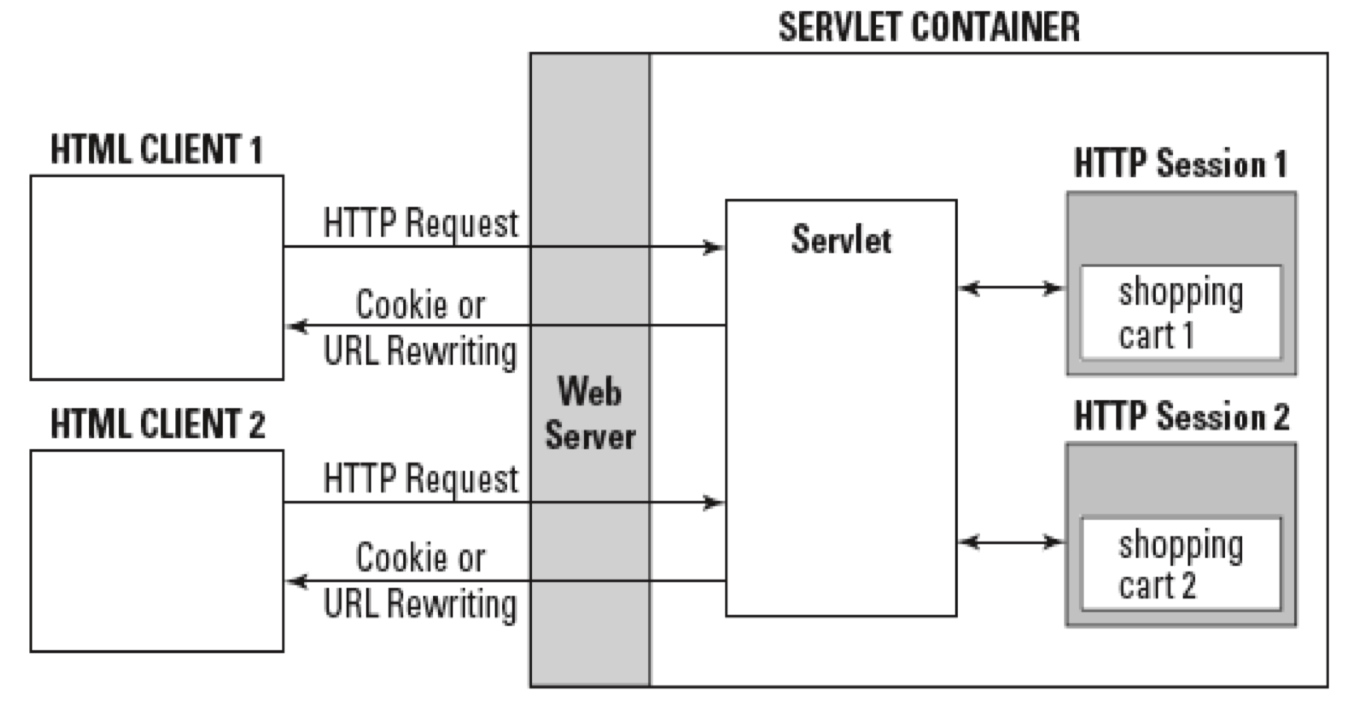
\includegraphics[width=0.6\textwidth]{fig_session.png}
  \end{figure}

  {\kai 每次HTTP请求时,所有Cookie会随求一起发送到Web服务器,保存在请求
    对象中。Web服务器从Cookie中得到SessionID,进而定位服务器内
    的HttpSession会话对象,实现Web的会话跟踪功能。}
\end{frame}

%%%%\begin{frame}[fragile] % [fragile]参数使得能够插入代码
%%%%\frametitle{Cookie方式} 
%%%%
%%%%HttpSession对象创建后,其{\hei SessionID会自动选择Cookie作为存储地},如果客户浏览器没有禁
%%%%止Cookie的读写,SessionID写入Cookie是不需要编程的,此项任务由Web容器自动完成。
%%%%\end{frame}
%%%%
%%%%\begin{frame}[fragile] % [fragile]参数使得能够插入代码
%%%%\frametitle{URL重写方式} 
%%%%
%%%%使用URL重写方式来保存和传递SessionID值,避免客户端浏览器的Cookie读写可能被禁止的情况。包含{\hei\Red 自动重定向和超链接重定向}。
%%%%
%%%%\tta{自动重定向}
%%%%
%%%%当使用{\hei\Red 响应对象}的sendRedirect方法实现自动重定向时,为保证地址URL中包含会话ID值,需要使用特定方式重写URL。
%%%%
%%%%Java Web响应对象提供将SessionID保存到URL的方法:
%%%%
%%%%\begin{javaCode}
%%%%public String encodeRedirectURL(String url);  
%%%%\end{javaCode}
%%%%
%%%%实现代码示例如下:
%%%%\begin{javaCode}
%%%%String url = response.encodeRedirectURL("main.jsp");
%%%%response.sendRedirect(url);
%%%%\end{javaCode}
%%%%
%%%%浏览器中URL显示如下:
%%%%\begin{shCode}
%%%%http://localhost:8080/MyFirstServlet/main.jsp;jsessionid=9FC729167DD922E3D978DC39EC2C19AA  
%%%%\end{shCode}
%%%%\end{frame}
%%%%
%%%%\begin{frame}[fragile] % [fragile]参数使得能够插入代码
%%%%\frametitle{URL重写方式} 
%%%%\tta{超链接重定向}
%%%%
%%%%使用超链接方式重定向导航时,也需要将导航目标地址进行URL重写,将SessionID封装到URL中,传递到目标页面。
%%%%\begin{javaCode}
%%%%public String encodeURL(String url);
%%%%\end{javaCode}
%%%%
%%%%实现代码示例如下:
%%%%\begin{javaCode}
%%%%String url = response.encodeURL("main.jsp");
%%%%PrintWriter out = response.getWriter();
%%%%...
%%%%out.println("<a href='" + url + "'>商城主页</a>");
%%%%... 
%%%%\end{javaCode}
%%%%\end{frame}

\begin{frame}[fragile] % [fragile]参数使得能够插入代码
  \frametitle{会话对象的应用示例} 

  \tta{保存用户的登录ID}

  \begin{javaCode}
    void doPost(HttpServletRequest request, HttpServletResponse response) {
      String userId = request.getParameter("userId");
      String password = request.getParameter("password");

      User user = BeanFactory.get("USER"); // 从Bean工厂获取一个User的对象实例
      
      if (user.validate(userId, password) { // 验证用户的有效性
        HttpSession session = request.getSession();  // 取得会话对象
        session.setAttribute("userId", userId);  // 将用户Id保存到会话对象
      } else { // 用户无效
        response.sendRedirect("../login.jsp"); // 重定向到登录页面
      }
    }
  \end{javaCode}
\end{frame}

\begin{frame}[fragile] % [fragile]参数使得能够插入代码
  \frametitle{会话对象的应用示例} 

  \tta{会话对象销毁(编程一般在注销功能中)}

  \begin{javaCode}
    public class LogoutAction extends HttpServlet {
      public void doGet(HttpServletRequest request, HttpServletResponse response) {
        HttpSession session = request.getSession();
        session.invalidate(); // 清除此会话对象
        response.sendRedirect("login.jsp"); // 跳转到登录页面
      }
    }
  \end{javaCode}
\end{frame}

\section{本节习题}

\begin{frame}
  \frametitle{本节习题}

  \tta{简答题}
  
  \begin{enumerate}
  \item 什么是会话跟踪?
  \item Java EE实现Web会话跟踪的方法有哪些?
  \item URL和Cookie实现会话跟踪的缺点分别有哪些?
  \item 简述使用Cookie和HTTP Session实现会话跟踪的机制。
  \end{enumerate}
\end{frame}

\begin{frame}[fragile]
  \frametitle{本节习题}
  
  \tta{小编程}

  实践课堂会话对象的应用实例,编写完整的用户登录、登录后才能浏览的主页,并在主页中包含登出按钮。

  \begin{enumerate}
  \item 登录页面为login.html,登录处理Servlet为LoginServlet.java,使用
    表单完成用户登录数据的提交并通过LoginServlet查询判断用户名和密码是
    否合法(可以硬编码,无需查询数据库),如用户名和密码合法则{\bf\Red
      重定向}到index.html。
    \begin{javaCode}
      if ("admin".equals(username) && "admin".equals(password)) {
        response.sendRedirect("index.html");
      } else {
        response.sendRedirect("login.html");
      }
    \end{javaCode}
  \item index.html中需要包含Logout按钮,用户点击Logout按钮则销毁当前会
    话并{\bf\Red 重定向}到login.html。
  \end{enumerate}
\end{frame}

% TKS %%%%%%%%%%%%%%%%%%%%%%%%%%%%%%%%%%%%%%%%%%%%%%
\begin{frame}
\centering
{\Huge \textcolor{blue}{THE END}} \\
\vspace{5mm}
{\Large wangxiaodong@ouc.edu.cn} \\
\end{frame}
%%%%%%%%%%%%%%%%%%%%%%%%%%%%%%%%%%%%%%%%%%%%%%%%%%
\end{document}
